%%%%%%%%%%%%%%%%%%%%%%%%%%%%%%%%%%%%%%%%% 
% Beamer Presentation
% LaTeX Template
% Version 1.0 (10/11/12)
% 
% This template has been downloaded from:
% http://www.LaTeXTemplates.com
% 
% License:
% CC BY-NC-SA 3.0 (http://creativecommons.org/licenses/by-nc-sa/3.0/)
% 
%%%%%%%%%%%%%%%%%%%%%%%%%%%%%%%%%%%%%%%%% 

% ----------------------------------------------------------------------------------------
%	PACKAGES AND THEMES
% ----------------------------------------------------------------------------------------

\documentclass{beamer}

\mode<presentation> {

  % The Beamer class comes with a number of default slide themes
  % which change the colors and layouts of slides. Below this is a list
  % of all the themes, uncomment each in turn to see what they look like.

  % \usetheme{default}
  % \usetheme{AnnArbor}
  % \usetheme{Antibes}
  % \usetheme{Bergen}
  % \usetheme{Berkeley}
  % \usetheme{Berlin}
  % \usetheme{Boadilla}
  % \usetheme{CambridgeUS}
  % \usetheme{Copenhagen}
  % \usetheme{Darmstadt}
  % \usetheme{Dresden}
  % \usetheme{Frankfurt}
  % \usetheme{Goettingen}
  % \usetheme{Hannover}
  % \usetheme{Ilmenau}
  \usetheme{JuanLesPins}
  % \usetheme{Luebeck}
  % \usetheme{Madrid}
  % \usetheme{Malmoe}
  % \usetheme{Marburg}
  % \usetheme{Montpellier}
  % \usetheme{PaloAlto}
  % \usetheme{Pittsburgh}
  % \usetheme{Rochester}
  % \usetheme{Singapore}
  % \usetheme{Szeged}
  % \usetheme{Warsaw}

  % As well as themes, the Beamer class has a number of color themes
  % for any slide theme. Uncomment each of these in turn to see how it
  % changes the colors of your current slide theme.

  % \usecolortheme{albatross}
  % \usecolortheme{beaver}
  % \usecolortheme{beetle}
  % \usecolortheme{crane}
  % \usecolortheme{dolphin}
  % \usecolortheme{dove}
  % \usecolortheme{fly}
  % \usecolortheme{lily}
  % \usecolortheme{orchid}
  % \usecolortheme{rose}
  % \usecolortheme{seagull}
  % \usecolortheme{seahorse}
  % \usecolortheme{whale}
  % \usecolortheme{wolverine}

  % \setbeamertemplate{footline} % To remove the footer line in all slides uncomment this line
  % \setbeamertemplate{footline}[page number] % To replace the footer line in all slides with a simple slide count uncomment this line

  % \setbeamertemplate{navigation symbols}{} % To remove the navigation symbols from the bottom of all slides uncomment this line
}

\usepackage{graphicx} % Allows including images
\usepackage{multirow}
\usepackage{booktabs} % Allows the use of \toprule, \midrule and \bottomrule in tables
\graphicspath{ {images/} }

% ----------------------------------------------------------------------------------------
%	TITLE PAGE
% ----------------------------------------------------------------------------------------

\title[OP platform introduction]{OP Platform Introduction} % The short title appears at the bottom of every slide, the full title is only on the title page

\author{Guanyu Yi} % Your name
\institute[Alchip] % Your institution as it will appear on the bottom of every slide, may be shorthand to save space
{
  OP Team, Alchip, Inc. \\ % Your institution for the title page
  \medskip
  \textit{guanyu\_yi@alchip.com} % Your email address
}
\date{\today} % Date, can be changed to a custom date

\begin{document}

\begin{frame}
  \titlepage % Print the title page as the first slide
\end{frame}

\begin{frame}
  \frametitle{Overview} % Table of contents slide, comment this block out to remove it
  \tableofcontents % Throughout your presentation, if you choose to use \section{} and \subsection{} commands, these will automatically be printed on this slide as an overview of your presentation
\end{frame}

% ----------------------------------------------------------------------------------------
%	PRESENTATION SLIDES
% ----------------------------------------------------------------------------------------

% ------------------------------------------------
\section{OP Platform Architecture} % Sections can be created in order to organize your presentation into discrete blocks, all sections and subsections are automatically printed in the table of contents as an overview of the talk

\begin{frame}
  \begin{figure}
    \centering
    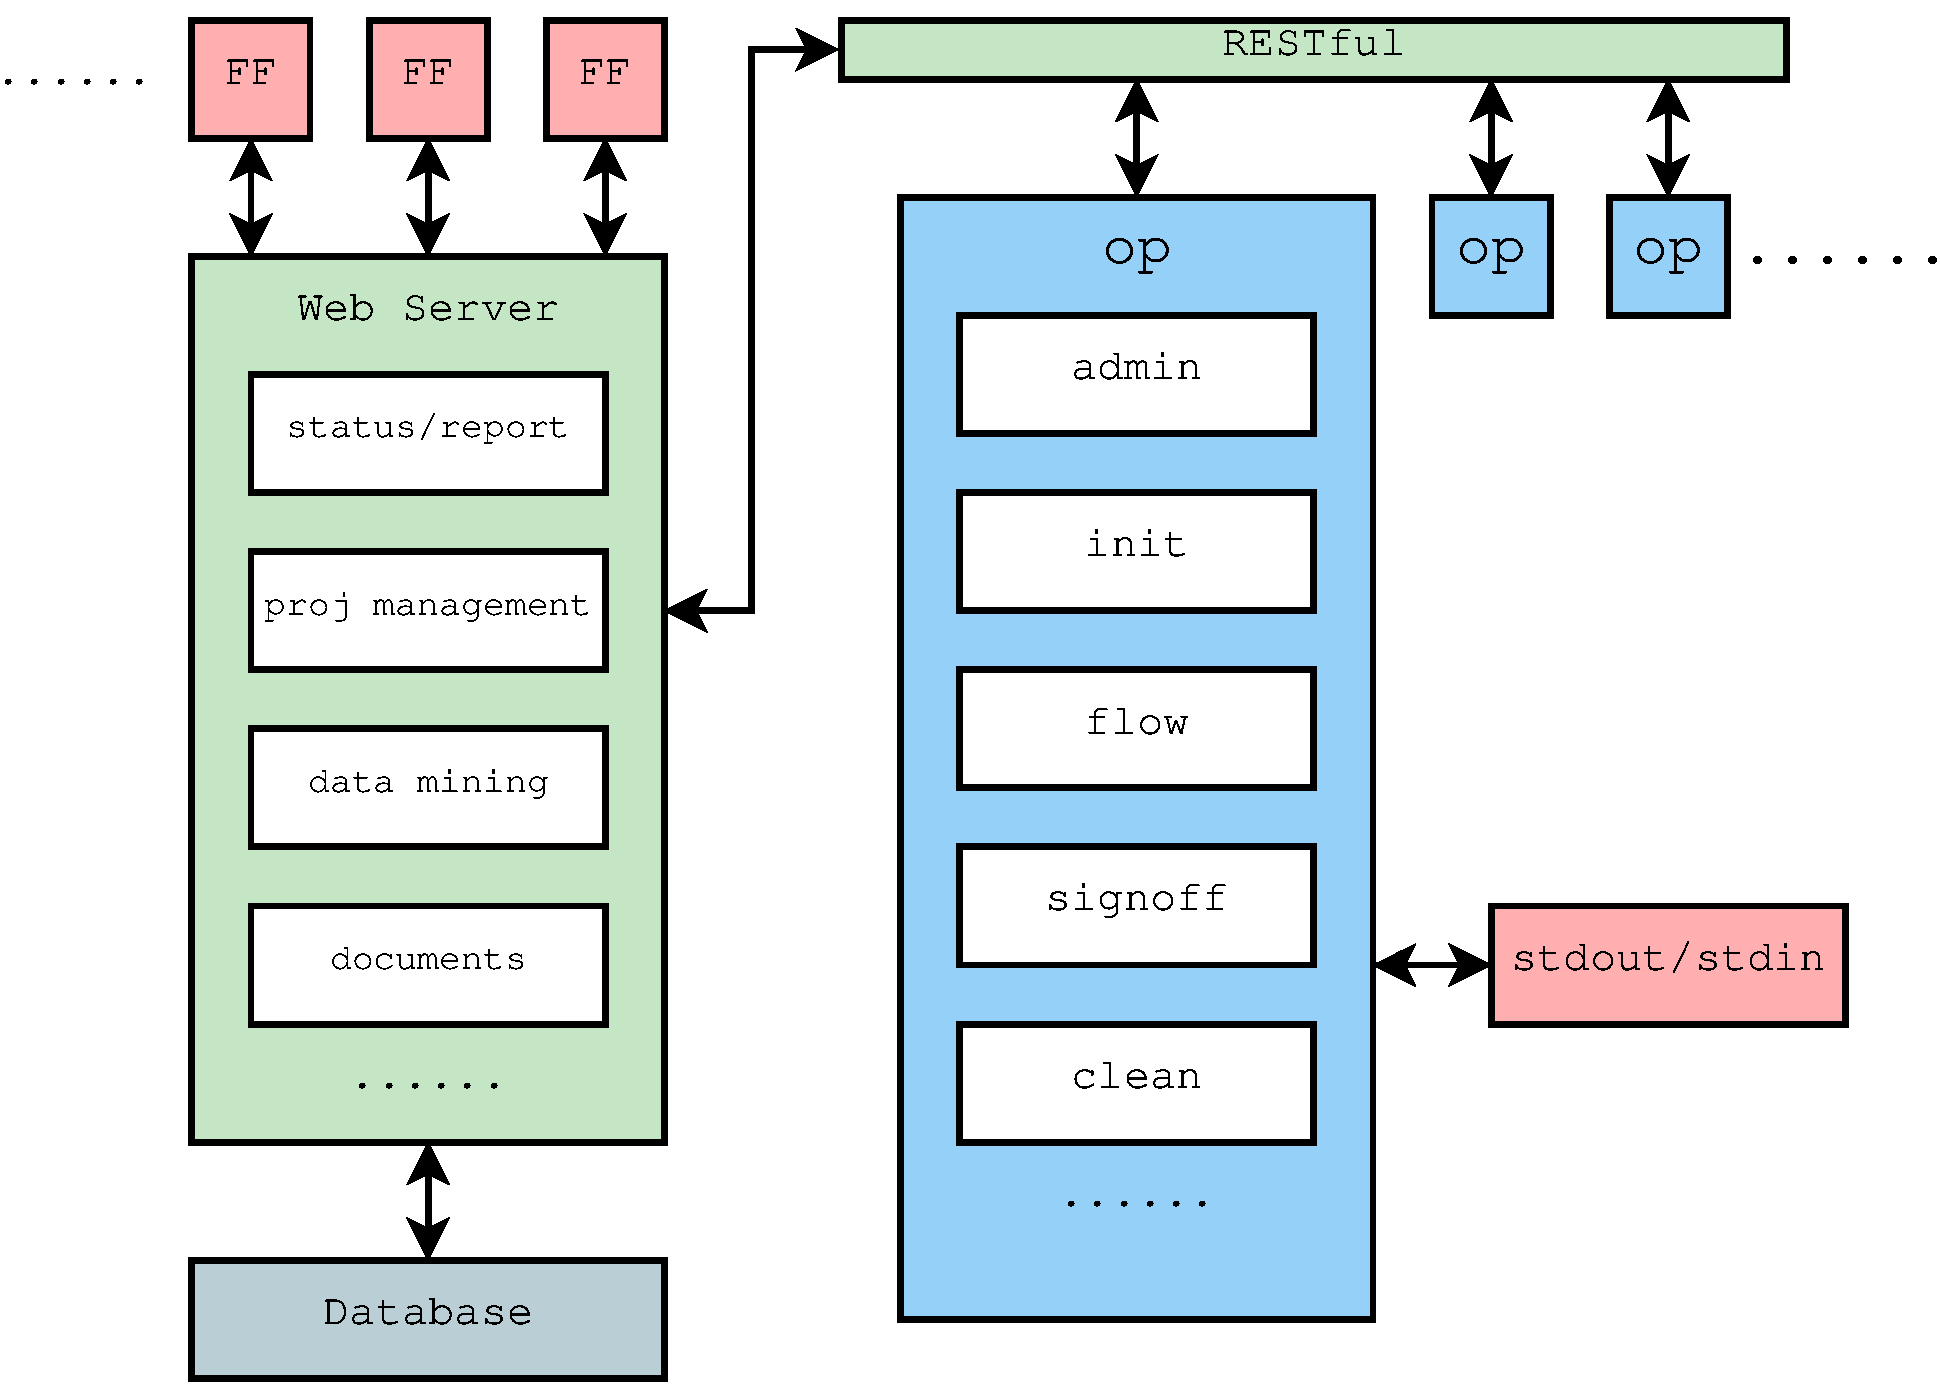
\includegraphics[width=0.98\linewidth]{pp_struc}
    \caption{Platform Architecture}
  \end{figure}
\end{frame}
% ----------------------------------------------------------------------------------------

% ------------------------------------------------
\section{Platform Runner Evolution} % Sections can be created in order to organize your presentation into discrete blocks, all sections and subsections are automatically printed in the table of contents as an overview of the talk

\begin{frame}
  \begin{figure}
    \centering
    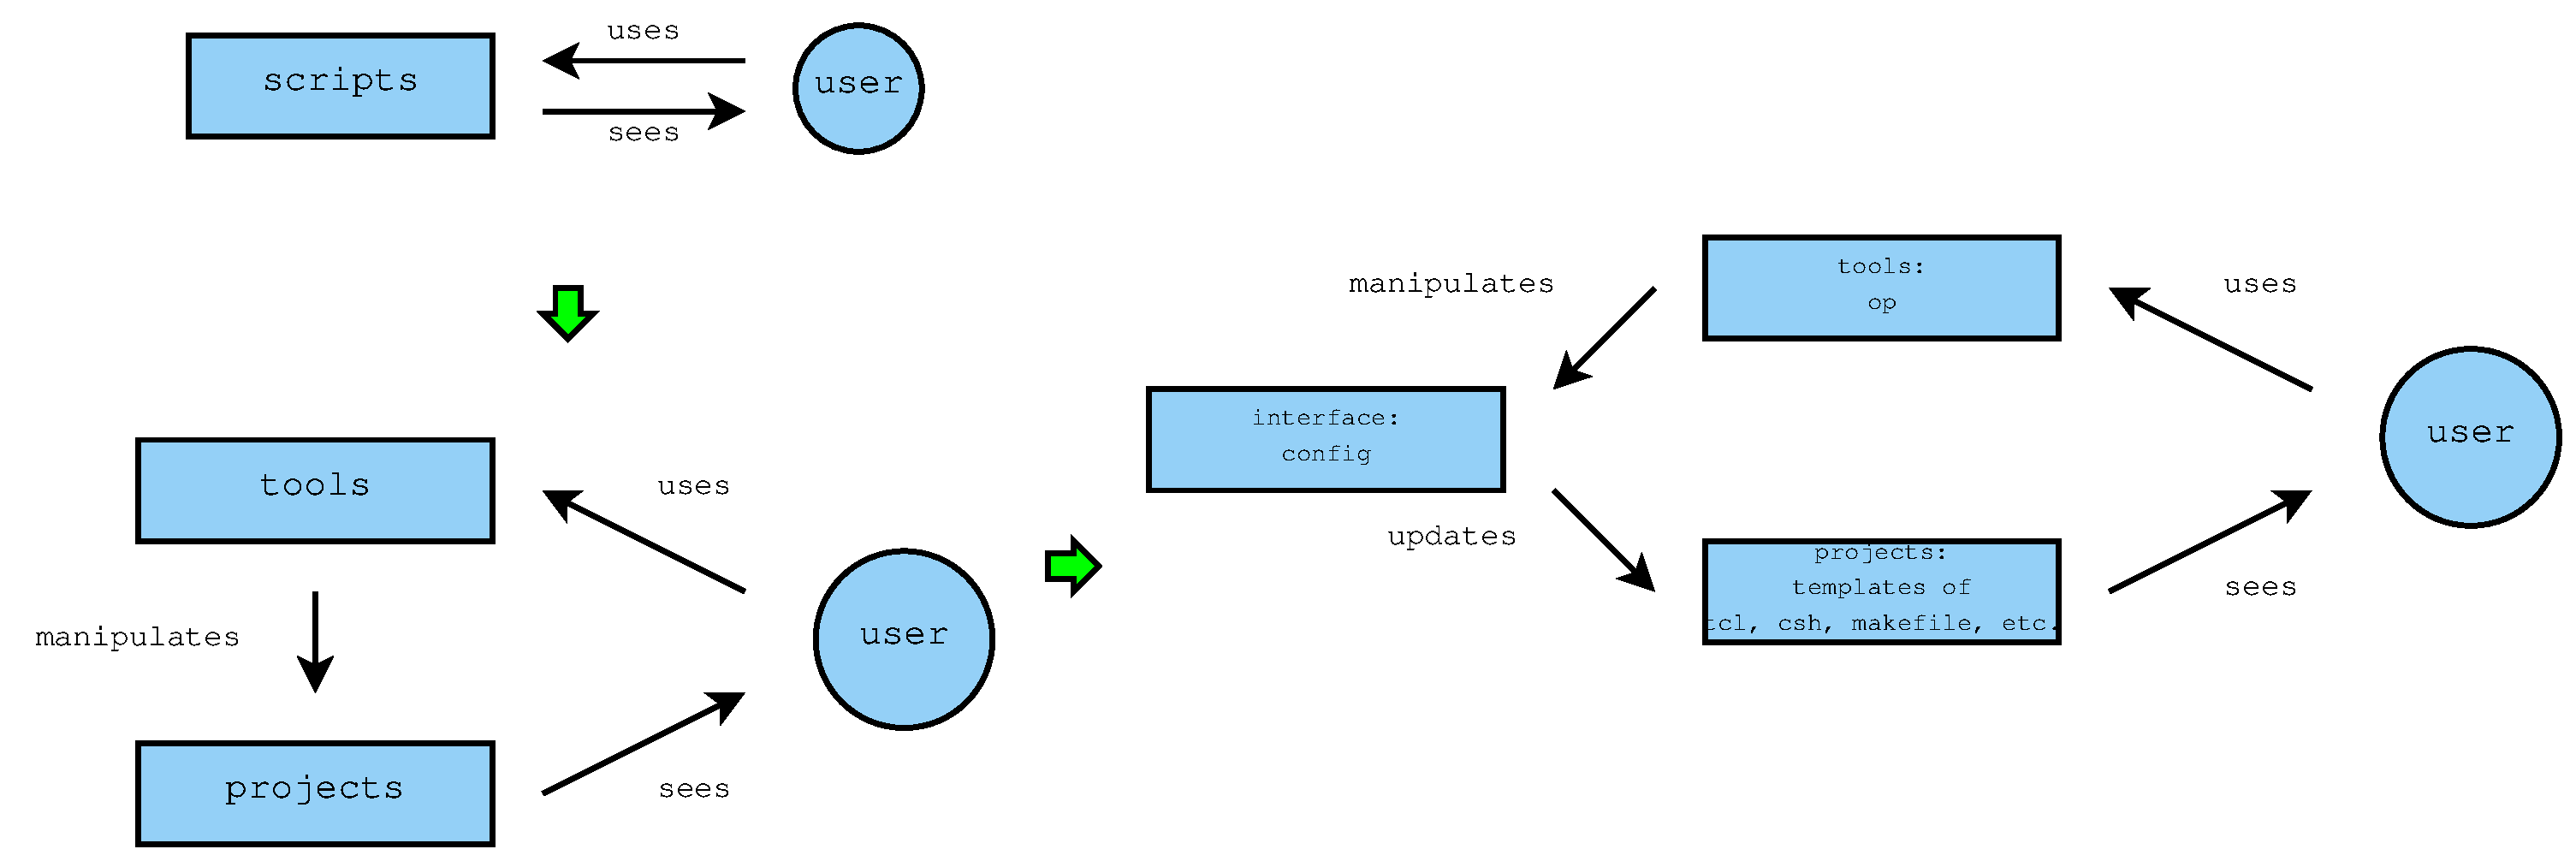
\includegraphics[width=1.05\linewidth]{mvc_evo}
    \caption{Platform Runner Evolution}
  \end{figure}
\end{frame}
% ----------------------------------------------------------------------------------------

% ------------------------------------------------
\section{MVC Framework} % Sections can be created in order to organize your presentation into discrete blocks, all sections and subsections are automatically printed in the table of contents as an overview of the talk

\begin{frame}
  \begin{columns}[c] % The "c" option specifies centered vertical alignment while the "t" option is used for top vertical alignment

    \column{.5\textwidth} % Right column and width
    \begin{figure}
      \centering
      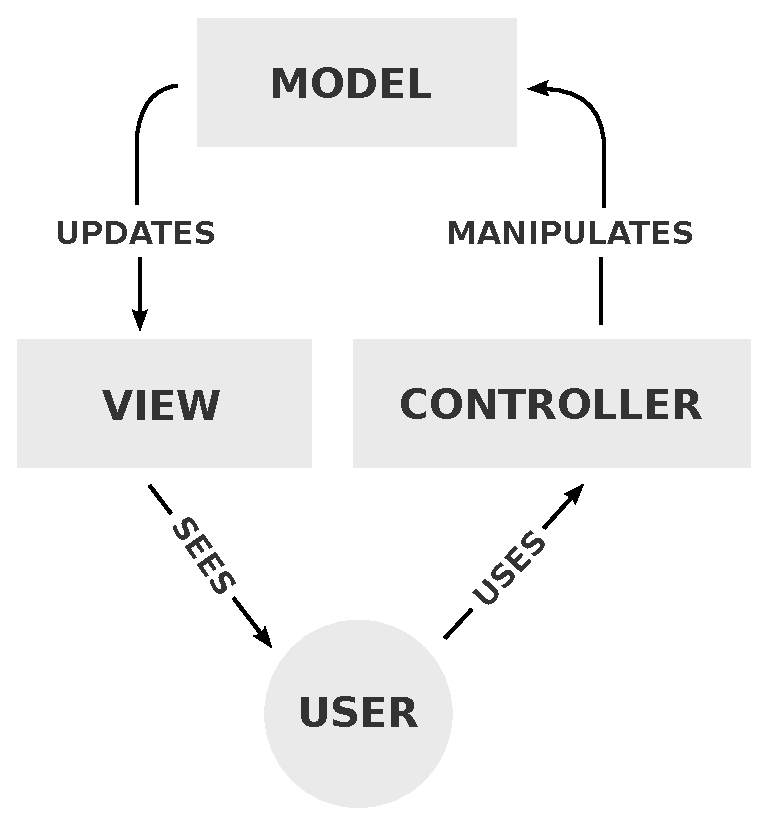
\includegraphics[width=0.75\linewidth]{mvc_process}
      \caption{MVC Framework}
    \end{figure}

    \column{.45\textwidth} % Left column and width
    \begin{enumerate}
    \item software architectural pattern
    \item decoupling major components
    \item runner is MVC style
    \end{enumerate}

  \end{columns}
\end{frame}
% ----------------------------------------------------------------------------------------

% ------------------------------------------------
\section{Platform Web Evolution} % Sections can be created in order to organize your presentation into discrete blocks, all sections and subsections are automatically printed in the table of contents as an overview of the talk

\begin{frame}
  \begin{figure}
    \centering
    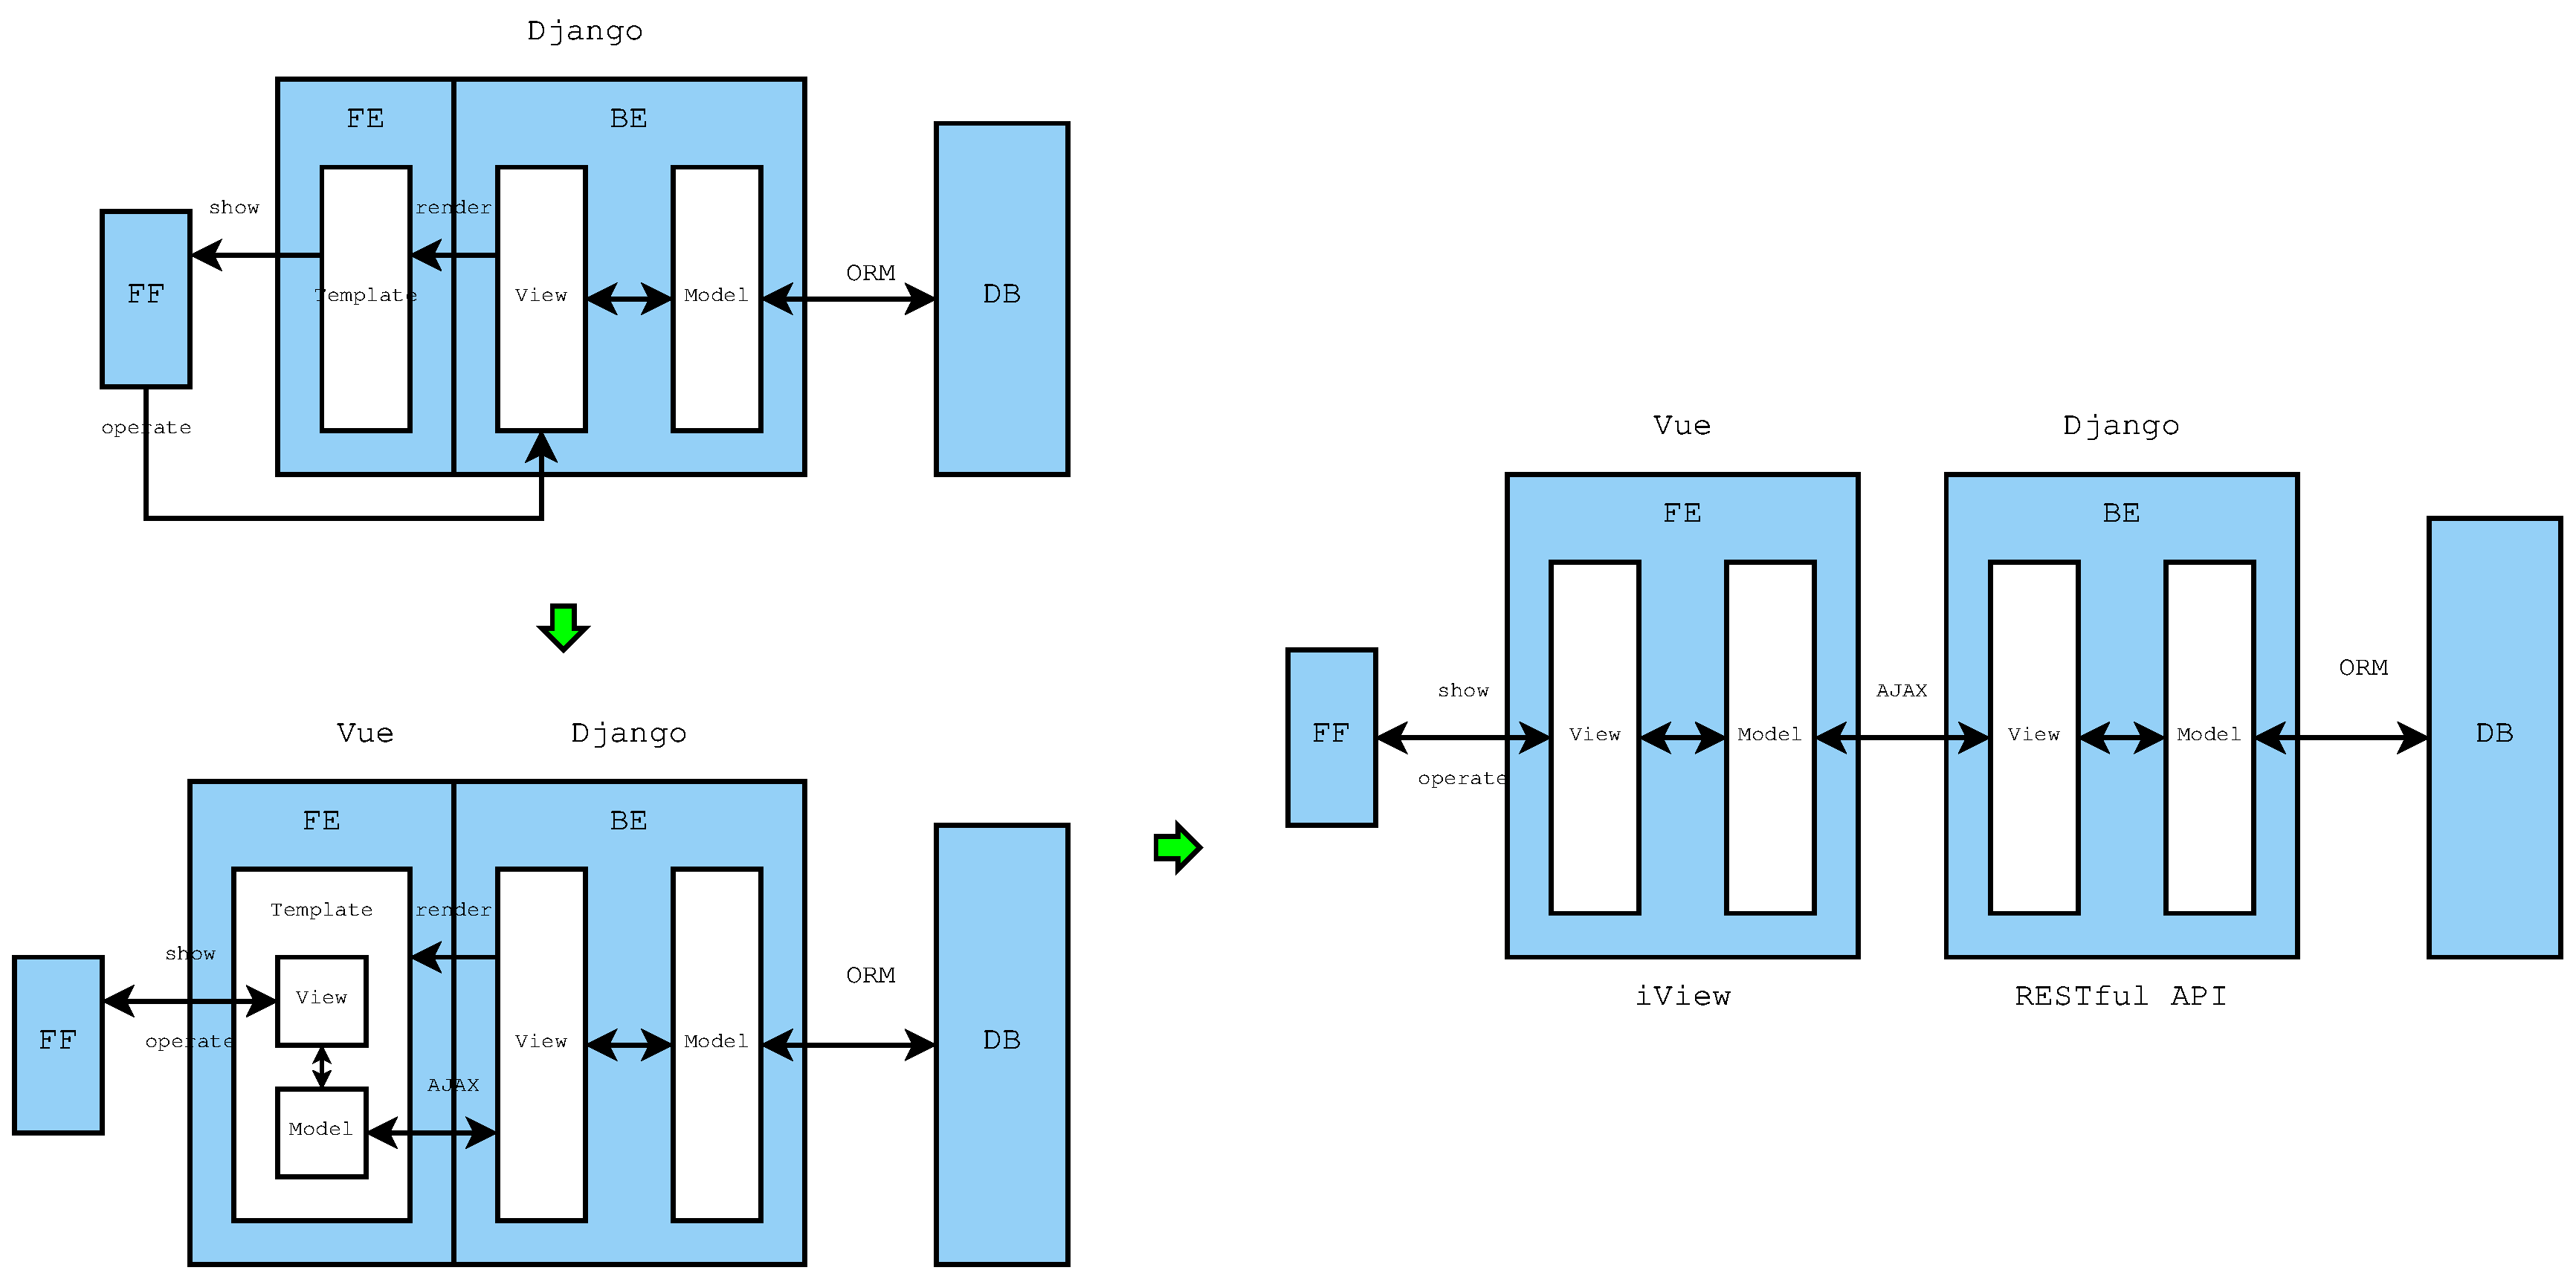
\includegraphics[width=1.05\linewidth]{web_evo}
    \caption{Platform Web Evolution}
  \end{figure}
\end{frame}
% ----------------------------------------------------------------------------------------

% ------------------------------------------------
\section{Project Hierarchy} % Sections can be created in order to organize your presentation into discrete blocks, all sections and subsections are automatically printed in the table of contents as an overview of the talk

\begin{frame}
  \begin{figure}
    \centering
    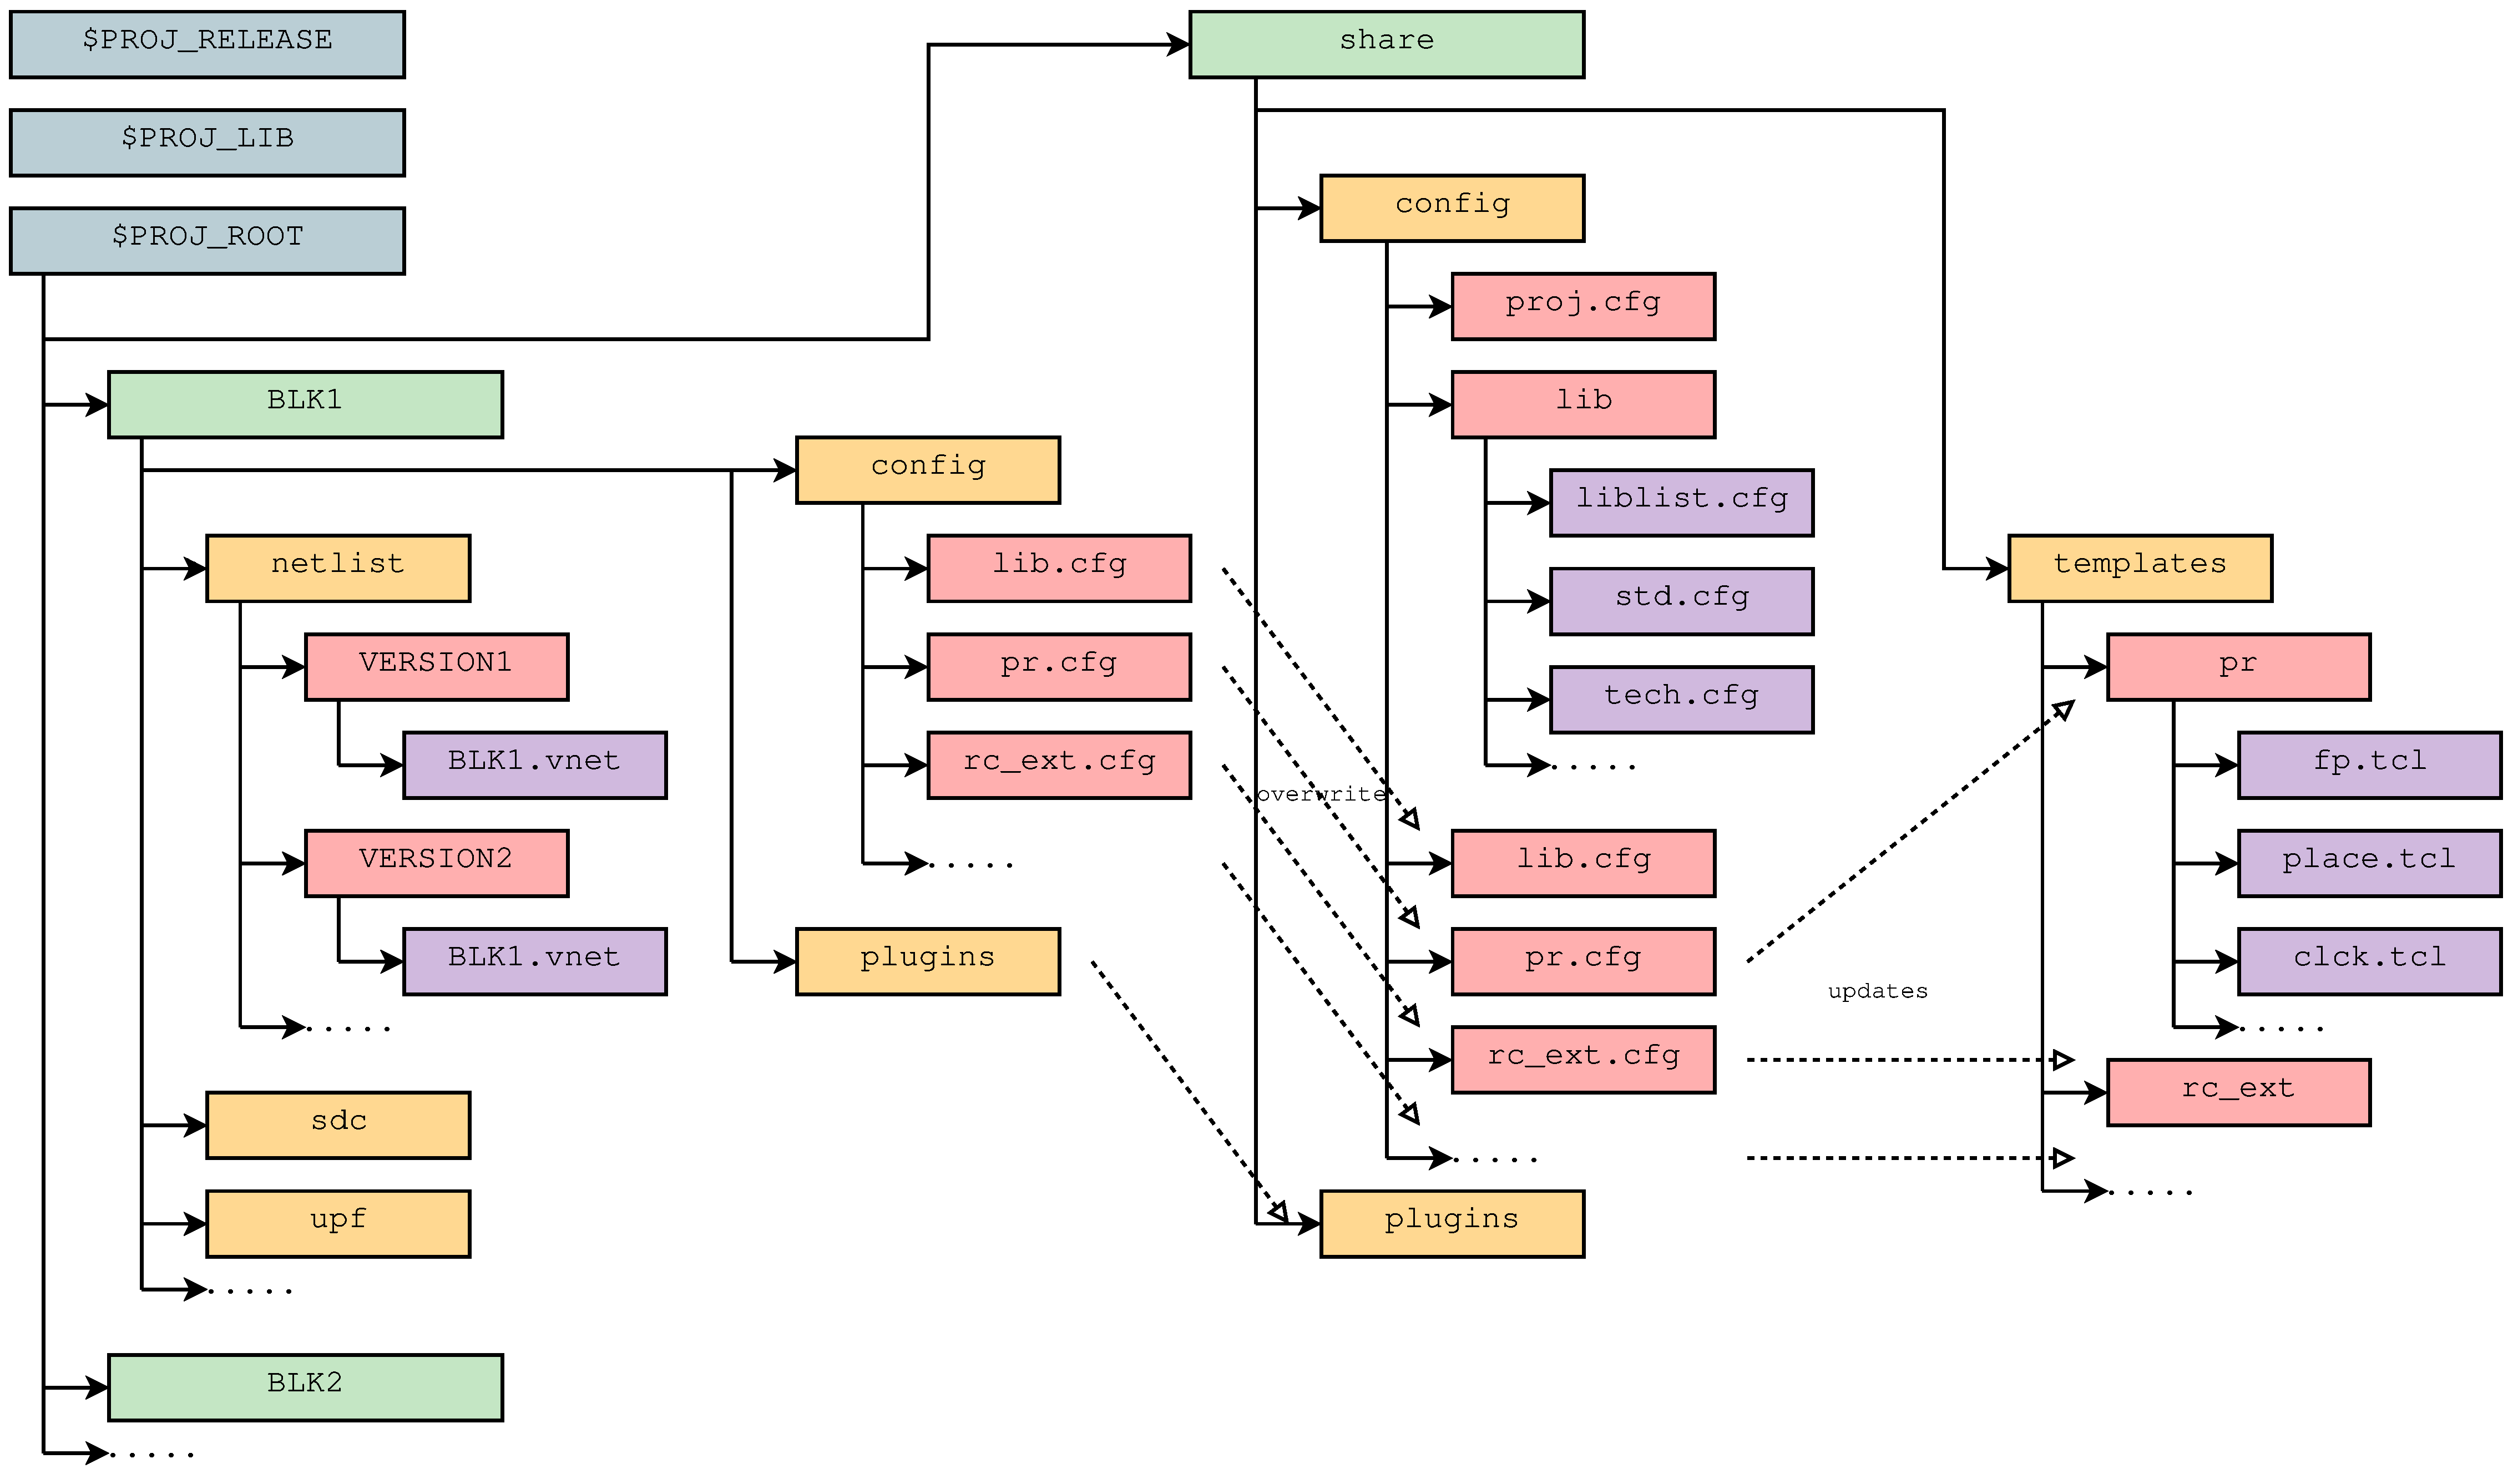
\includegraphics[width=1.05\linewidth]{proj_hier}
    \caption{Project Hierarchy, Config and Templates}
  \end{figure}
\end{frame}
% ----------------------------------------------------------------------------------------

% ------------------------------------------------
\section{Config and Templates} % Sections can be created in order to organize your presentation into discrete blocks, all sections and subsections are automatically printed in the table of contents as an overview of the talk

\begin{frame}
  \begin{columns}[c] % The "c" option specifies centered vertical alignment while the "t" option is used for top vertical alignment

    \column{.45\textwidth} % Left column and width
    \textbf{Config}
    \begin{enumerate}
    \item INI vs JSON/XML
    \item Sections and Options
    \item Default Overwritten
    \end{enumerate}

    \column{.45\textwidth} % Left column and width
    \textbf{Templates}
    \begin{enumerate}
    \item Python Jinja2 Engine
    \item Programmable (condition and loop)
    \item Extensible (include and extend)
    \end{enumerate}

  \end{columns}
\end{frame}
% ----------------------------------------------------------------------------------------

% ------------------------------------------------
\section{Library Mapping} % Sections can be created in order to organize your presentation into discrete blocks, all sections and subsections are automatically printed in the table of contents as an overview of the talk

\begin{frame}
  \begin{figure}
    \centering
    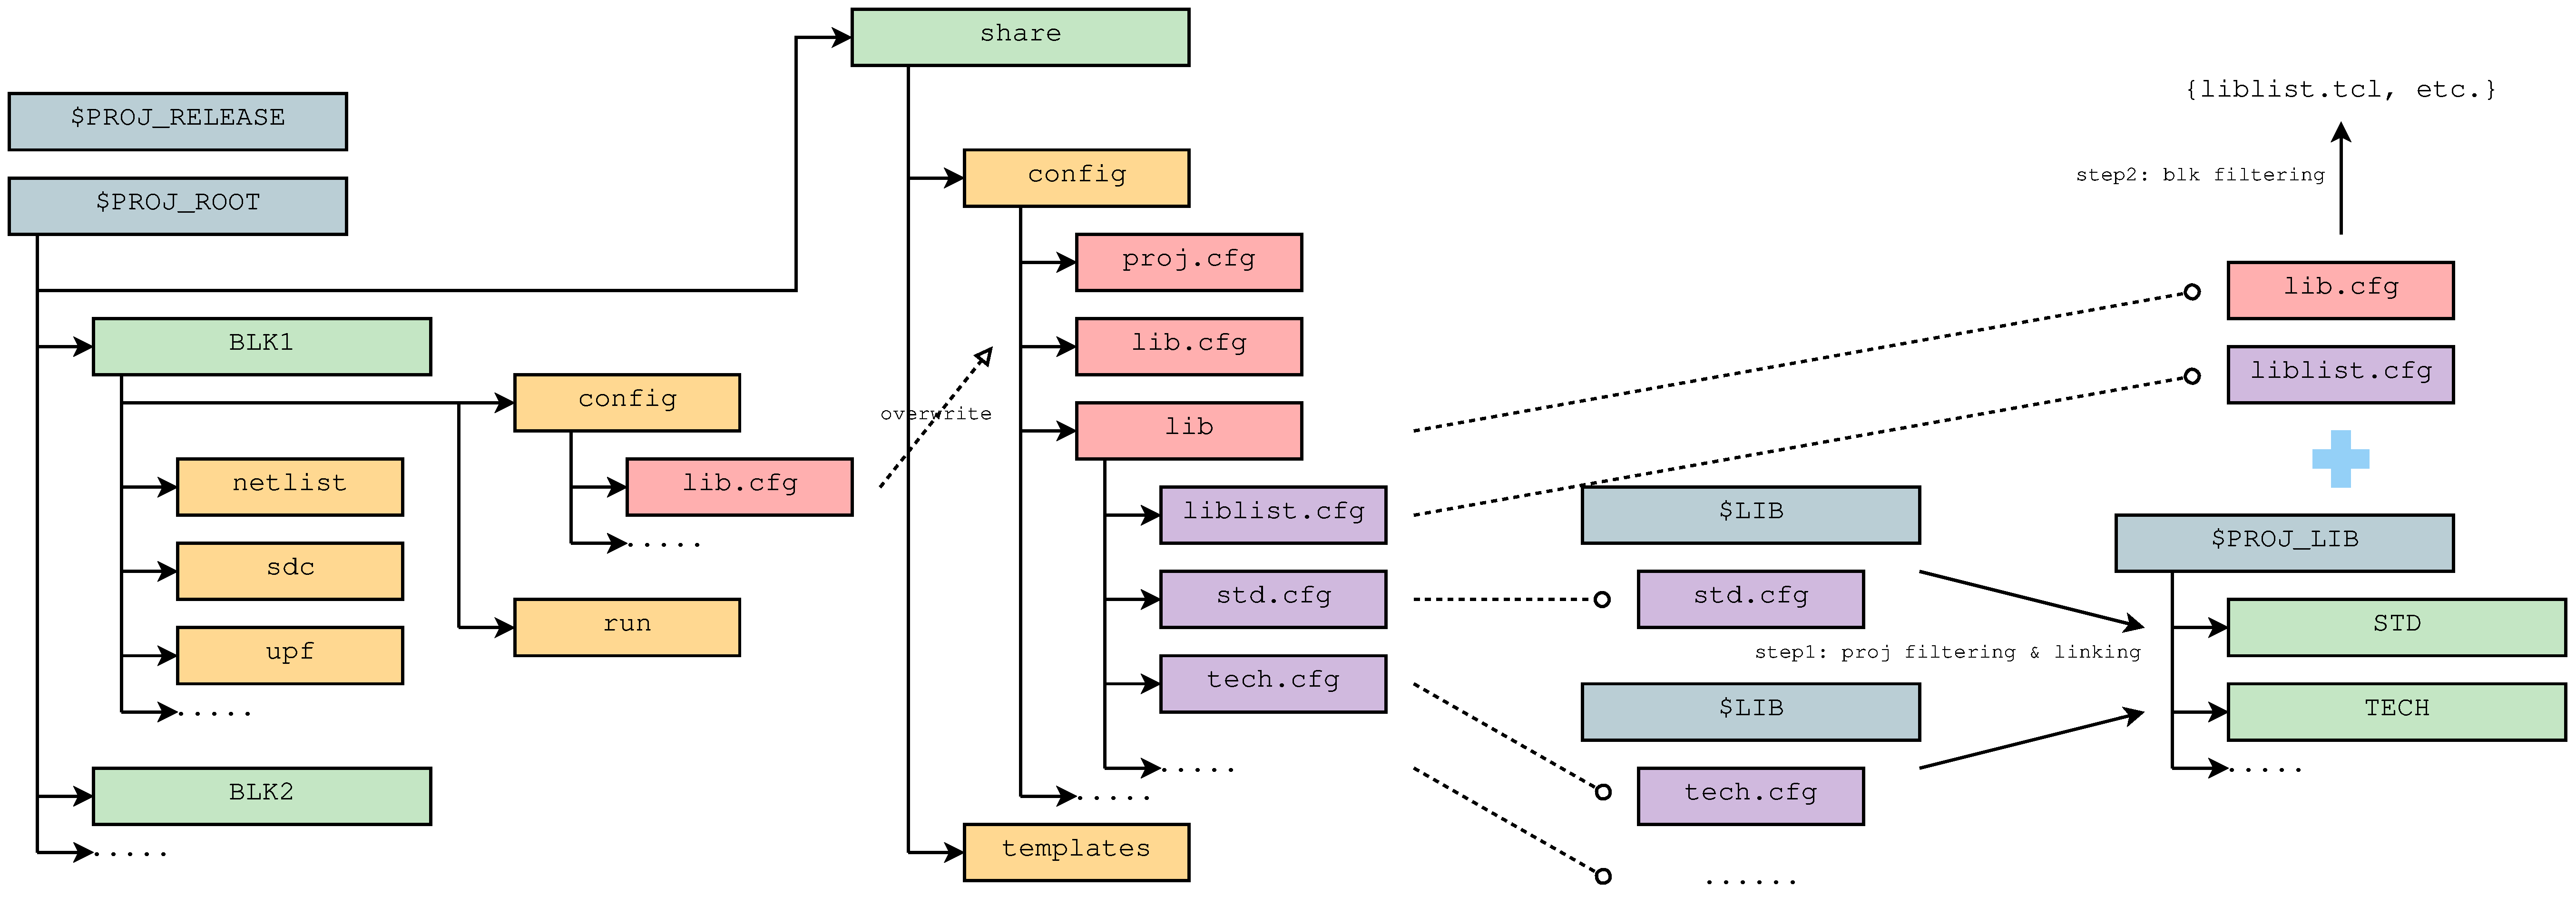
\includegraphics[width=1.10\linewidth]{lib_map_hier}
    \caption{Library Mapping Procedure}
  \end{figure}
\end{frame}
% ----------------------------------------------------------------------------------------

% ------------------------------------------------
\section{Flow Running} % Sections can be created in order to organize your presentation into discrete blocks, all sections and subsections are automatically printed in the table of contents as an overview of the talk

\begin{frame}
  \begin{figure}
    \centering
    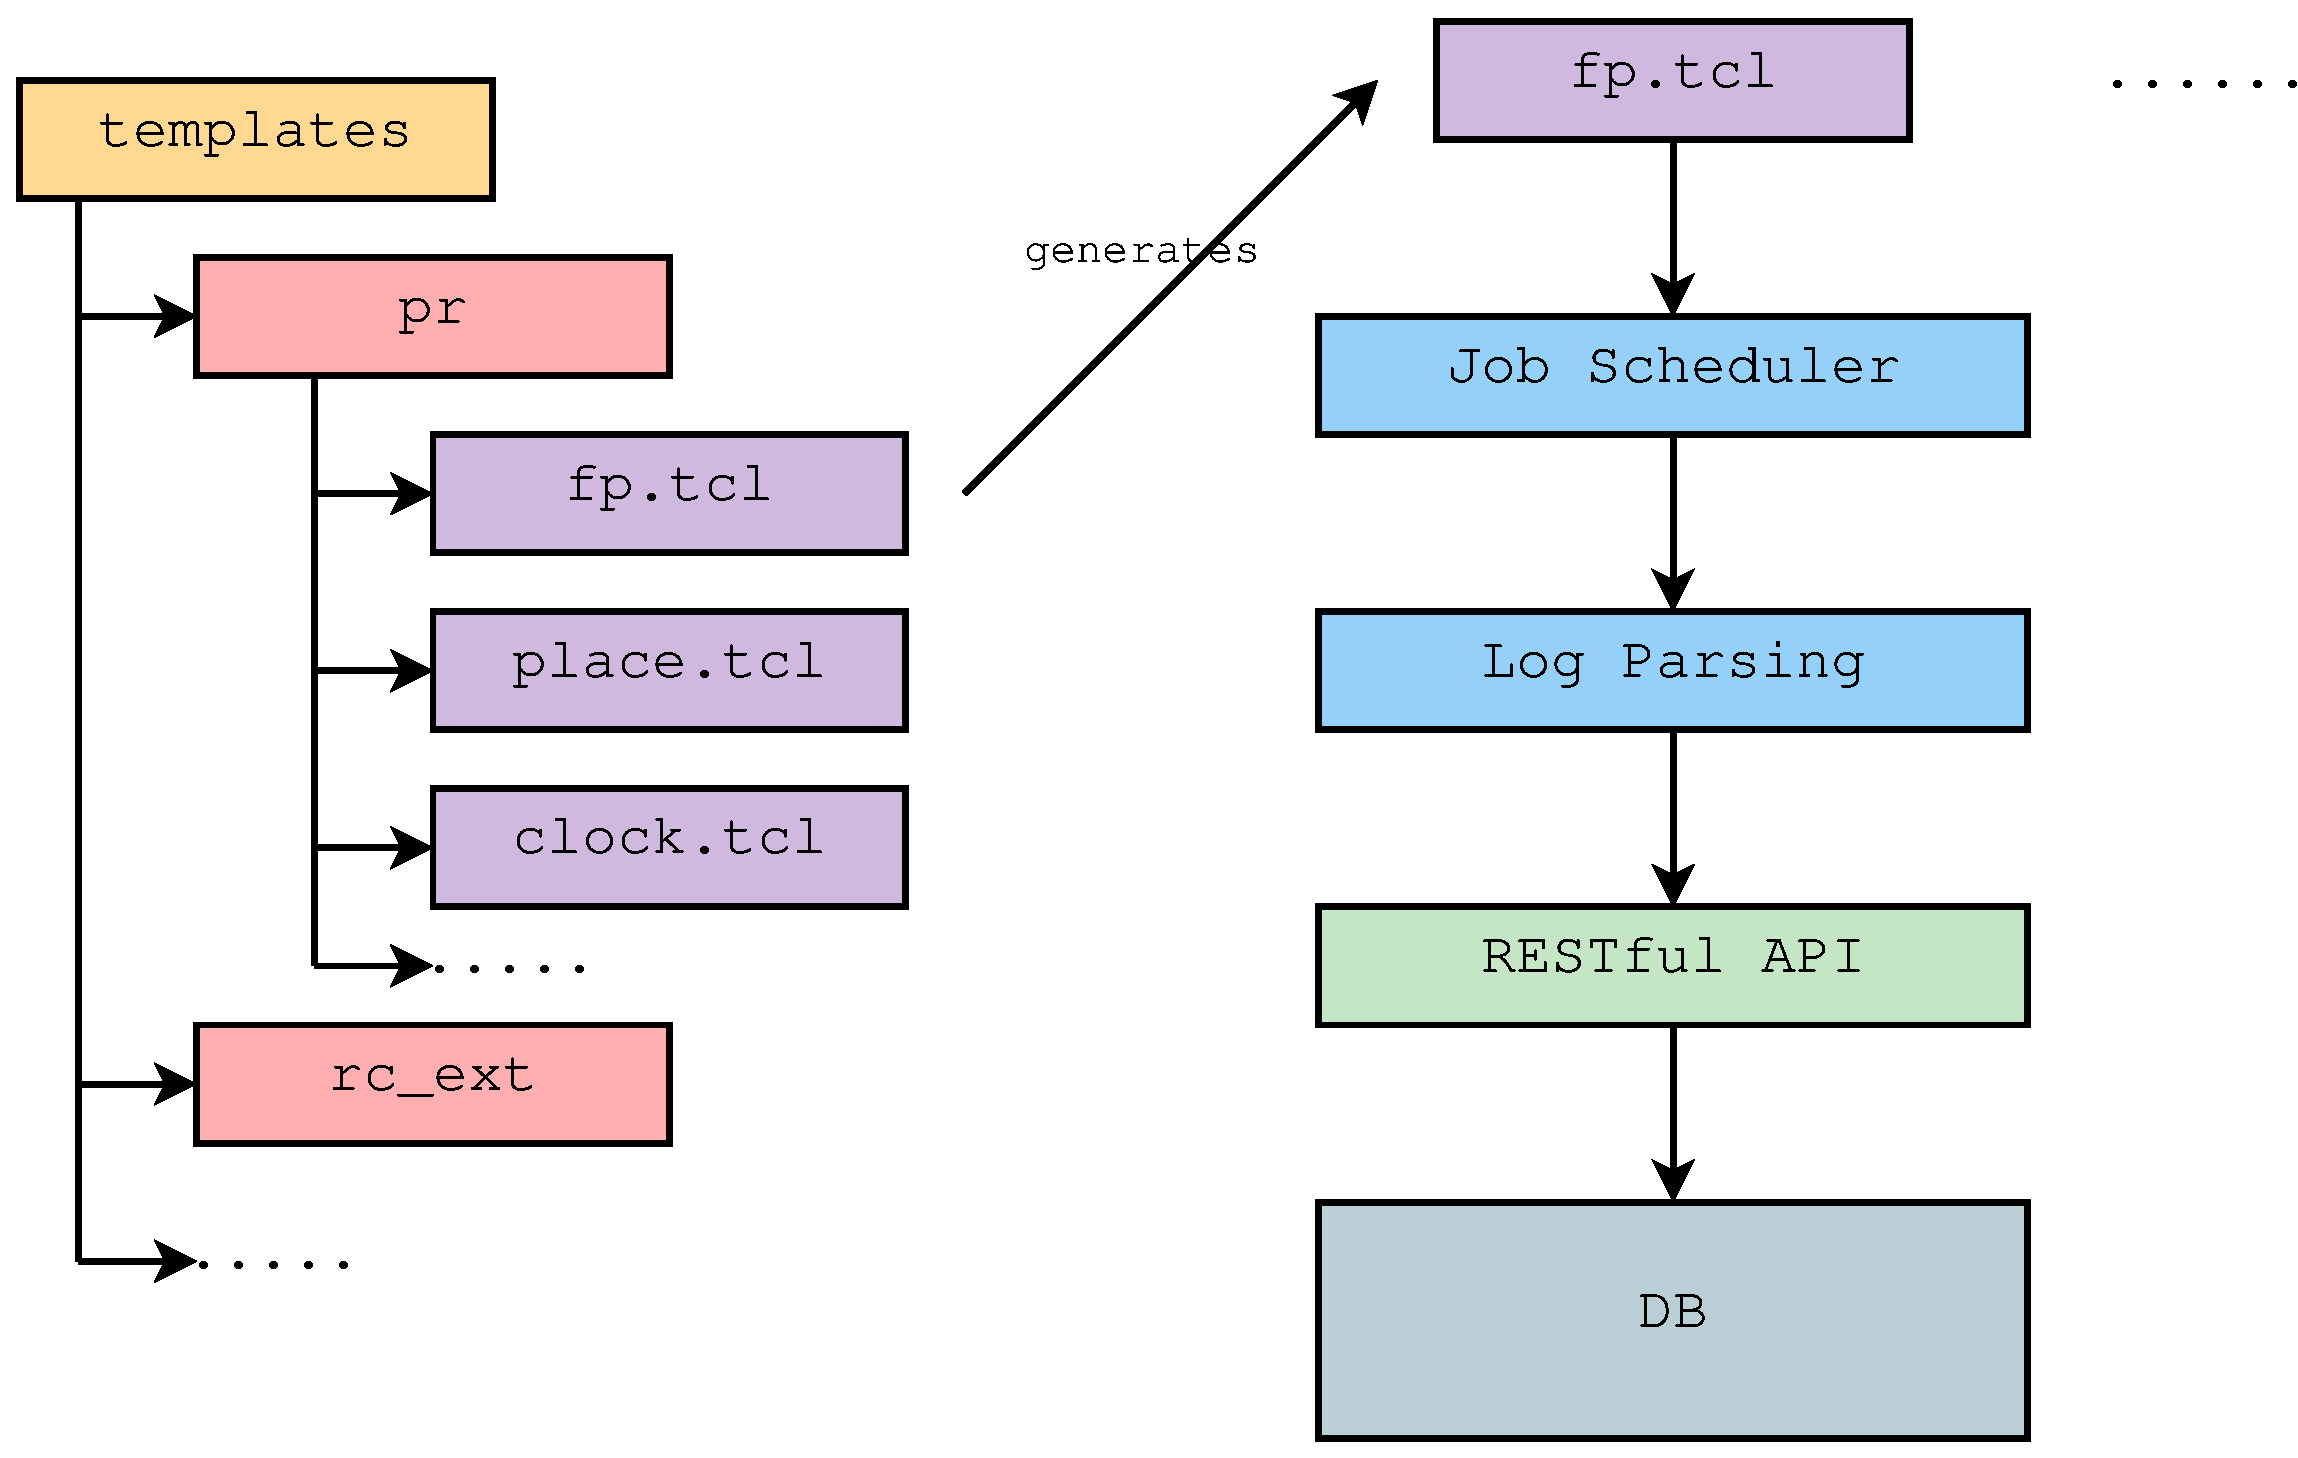
\includegraphics[width=0.80\linewidth]{flow_proc}
    \caption{Flow Running Procedure}
  \end{figure}
\end{frame}
% ----------------------------------------------------------------------------------------

% ----------------------------------------------------------------------------------------

\begin{frame}
  \Huge{\centerline{Q \& A}}
\end{frame}

% ----------------------------------------------------------------------------------------

\end{document} 
%%% Local Variables:
%%% mode: latex
%%% TeX-master: t
%%% End:
